\documentclass{beamer}

\mode<presentation>
{
  \usetheme{Singapore}
  \usecolortheme{rose}
  \setbeamercovered{transparent}
}

\usepackage[english]{babel}
\usepackage[latin1]{inputenc}
\usepackage{times}
\usepackage{listings}
\usepackage[T1]{fontenc} 
\usepackage{caption}

% Or whatever. Note that the encoding and the font should match. If T1
% does not look nice, try deleting the line with the fontenc.
\usepackage{amsmath}
\newcommand{\linespace}{\vskip 0.25cm}

\definecolor{MyForestGreen}{rgb}{0,0.7,0} 
\newcommand{\tableemph}[1]{{#1}}
\newcommand{\tablewin}[1]{\tableemph{#1}}
\newcommand{\tablemid}[1]{\tableemph{#1}}
\newcommand{\tablelose}[1]{\tableemph{#1}}

\definecolor{MyLightGray}{rgb}{0.6,0.6,0.6}
\newcommand{\tabletie}[1]{\color{MyLightGray} {#1}}

\beamertemplatenavigationsymbolsempty

\addtobeamertemplate{navigation symbols}{}{%
    \usebeamerfont{footline}%
    \usebeamercolor[fg]{footline}%
    \hspace{1em}%
    \insertframenumber/\inserttotalframenumber
}

\lstset{language=Java, frame=single, showspaces=false, }

\title[Developmental plasticity in N-gram GP]{Thread Scheduler Efficiency Improvements \\ for Multicore Systems}

% Sub-titles are optional - uncomment and edit the next line if you want one.
% \subtitle{Why does sub-tree crossover work?} 

% The text in square brackets is the short version of your name(s) and will be used in the
% header/footer depending on your theme.
\author[DFrz]{Daniel Collin Frazier}

% The text in square brackets is the short version of your institution and will be used in the
% header/footer depending on your theme.
\institute[U of Minn, Morris]
{
  Division of Science and Mathematics \\
  University of Minnesota, Morris \\
  Morris, Minnesota, USA
}

% The text in square brackets is the short version of the date if you need that.
\date[November '17, UMM, Minnesota] % (optional)
{18 November 2017 \\ UMM, Minnesota}

% Delete this, if you do not want the table of contents to pop up at
% the beginning of each subsection:
\AtBeginSection[]
{
	\begin{frame}<beamer>
		\frametitle{Outline}
		\tableofcontents[currentsection, hideothersubsections]
	\end{frame}
}

\begin{document}

\begin{frame}
\titlepage
\end{frame}

% For a 20-25 minute senior seminar talk you probably want something like:
% - Two or three major sections (other than the summary).
% - At *most* three subsections per section.
% - Talk about 30s to 2min per frame. So there should probably be between
%   15 and 30 frames, all told.

\section*{Introduction}

\subsection*{Introduction}

\begin{frame}
  \frametitle{Introduction}
  
\begin{itemize}
	\item \emph{Thread scheduler} is an important system component that manages the processing programs receive in a given time
  	\item Always running, so it must be efficient
  	
	\linespace
	
 	\item Most computers before 2001 were equipped with one processor containing one core
	\item At the end of the single-processor single-core era (early 2000s) thread scheduling was largely considered a solved problem by the Linux community

\end{itemize}

\end{frame}


\begin{frame}

\begin{figure}

\begin{quote}
``...not very many things ... have aged as well as the scheduler. Which is just another proof that scheduling is easy.''
\end{quote}
Linus, Torvals, 2001 \cite{Lozi:2016}
\end{figure}
\end{frame}

\begin{frame}
\frametitle{Introduction}

Popular hardware changed rapidly throughout the 2000s and those developments made thread scheduler implementation much more complex

\linespace

One of these driving changes was the increasing affordability and adoption of multicore systems

\linespace

Unfortunately, this increasing complexity led to bugs

\end{frame}

\begin{frame}
\frametitle{A Decade of Wasted Cores}

\begin{columns}
\begin{column}{0.72\textwidth}
Lozi et al. found four bugs in the Linux thread scheduler and fixed them~\cite{Lozi:2016}

\linespace

Undetected by pre-existing diagnostic tools, required the development of new tools to notice them

\linespace
\begin{itemize}
	\item The Scheduling Group Construction bug
	\item The Group Imbalance bug
	\item The Overload-on-Wakeup bug
	\item The Missing Scheduling Domains bug
\end{itemize}
\end{column}
\begin{column}[b]{0.28\textwidth} %Why does to[p] make the figure on the bottom and [b]ottom make the figure on the top.....
\begin{figure}
\centering
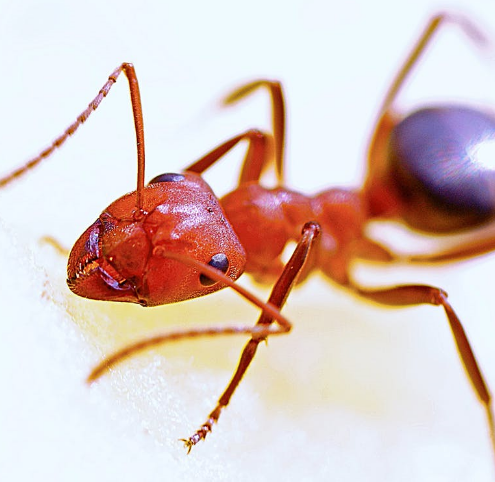
\includegraphics[width=0.95\textwidth]{Illustrations/ant_from_pexels.png}
\caption*{https://goo.gl/3wsfVU}
\end{figure}
\end{column}
\end{columns}
\end{frame}

\begin{frame}
\frametitle{Scheduling Group Construction bugfix results}

To gauge improved efficiency, Lozi et al. used a group of 9 computational applications that heavily utilize threads called the \emph{NAS Parallel Benchmark (NPB)}, developed by NASA

\begin{table}
	\centering
	\begin{tabular}{| c | c | c | c |}
		\hline			
	  	Application & Time w/ bug (sec) & Time w/o bug (sec) & Speedup factor (x) \\ \hline
		is & 271 & 202 & 1.33 \\ \hline
		mg & 49 & 24 & 2.03 \\ \hline
		lu & 1040 & 38 & 27 \\ \hline
		\hline
	\end{tabular}
	\caption{"NPB applications with least, median and most improvement between a bugged and fixed scheduler"~\cite{Lozi:2016}}
\end{table}

\end{frame}

\begin{frame}
\frametitle{Group Imbalance and Overload-on-Wakeup bugfixes}
\begin{table}
	\centering
	\begin{tabular}{| c | c | c |}
		\hline			
	  	Bug Fixes & TPC-H request \#18 & Full TPC-H benchmark \\ \hline
		\emph{None} & 55.9s & 542.9s \\ \hline
		\emph{Group Imbalance} & 48.6s (-13.1\%) & 512.8s (-5.4\%) \\
		\emph{Overload-on-Wakeup} & 43.5s (-22.2\%) & 471.1s (-13.2\%) \\
		\emph{Both} & 43.3s (-22.6\%) & 465.6s (-14.2\%) \\
		\hline
	\end{tabular}
	\caption{"Impact of these bug fixes on a popular commercial database (values averaged after five runs.)"~\cite{Lozi:2016}}
\end{table}

They disabled and re-enabled a core before each run of the benchmark
\end{frame}

\begin{frame}
\frametitle{Missing Scheduling Domain bugfix results}

Occurs rarely, but easily reproducible

\begin{table}
	\centering
	\begin{tabular}{| c | c | c | c |}
		\hline			
	  	Application & Time w/ bug (sec) & Time w/o bug (sec) & Speedup factor (x) \\ \hline
		ep & 72 & 18 & 4.0 \\ \hline
		mg & 81 & 9 & 9.03 \\ \hline
		lu & 2196 & 16 & 137.59 \\ \hline	
		\hline
	\end{tabular}
	\caption{"NPB applications with least, median and most improvement between a bugged and fixed scheduler"~\cite{Lozi:2016}}
\end{table}
\end{frame}



\subsection*{Outline}

\begin{frame}
  \frametitle{Outline}
  \tableofcontents[hideallsubsections]
\end{frame}

\section[Concepts]{Concepts}

\subsection[Threads]{Threads}

\begin{frame}
\frametitle{Introduction}
	\begin{itemize}
	\item The computer processor is responsible for executing compiled code.
		\item A single-core processor has one \emph{processing unit}, while a multi-core processor has many \emph{processing units}.

	\item A processor with multiple cores allows it to perform tasks concurrently on each core
	\end{itemize}
\end{frame}

\begin{frame}
\frametitle{Using Threads}

\begin{columns}
	\begin{column}{0.5\textwidth}
		\emph{Threads} allow a program to run multiple independent tasks at the same time

		\linespace
		\begin{itemize}
		\item Imagine you're using photoshop but it has one thread
		\item You load a large image and perform an expensive filter operation
		\end{itemize}
		\end{column}
	\begin{column}{0.5\textwidth}
		\begin{figure}
		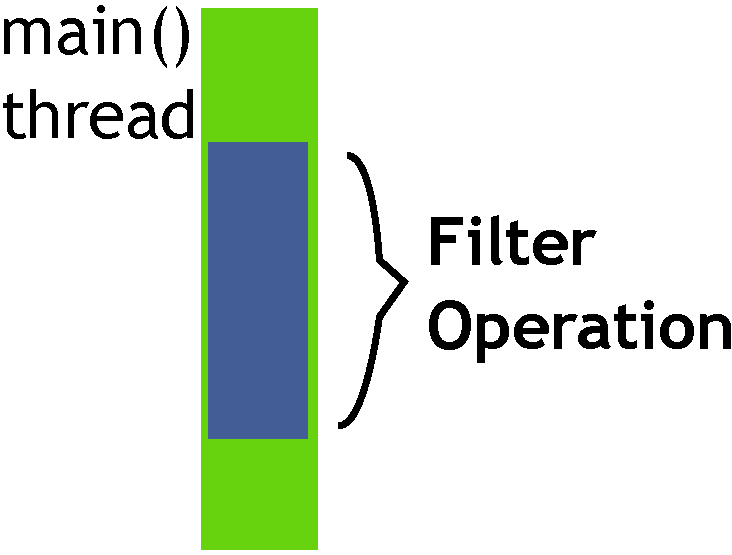
\includegraphics[width=0.95\textwidth]{Illustrations/ThreadExample_GUI_Part1}
		\label{fig:domains}
		\caption{Running a filter operation in a hypothetical single-threaded version of photoshop}
		\end{figure}
	\end{column}
\end{columns}

\end{frame}

\begin{frame}
\frametitle{Using Threads}

\begin{columns}
	\begin{column}{0.5\textwidth}
		\begin{itemize}
		
		\linespace
		
		\item Useful for programs:
			\begin{itemize}
  			 \item with long, mostly-independent computations
			 \item with a graphical interface
	  		\end{itemize}
		\end{itemize}
	\end{column}
	
	\begin{column}{0.5\textwidth}
		\begin{figure}
		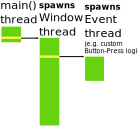
\includegraphics[width=0.95\textwidth]{Illustrations/ThreadExample_GUI_Part2}
		\label{fig:domains}
		\caption{Example GUI Program. \textbf{Three} threads are created within \textbf{one} process}
		\end{figure}
	\end{column}
\end{columns}

\end{frame}

\begin{frame}
\frametitle{Race Conditions}

One problem multithreaded programs face are called \emph{Race~Conditions}

\linespace

Defined in Saltzer and Kaashoek as ``A timing-dependent error in thread coordination that may result in threads computing incorrect results'' 

\linespace

Let's see an example where two threads increment a shared variable
\end{frame}

\begin{frame}
\frametitle{Race Condition Example}
	\begin{figure}
		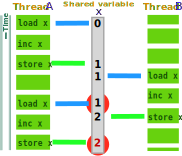
\includegraphics[width=0.8\textwidth]{Illustrations/RaceCondition}
		\label{fig:racecondition}
	\end{figure}

\end{frame}

\subsection[Locks]{Synchronicity and Locks}


\begin{frame}
\frametitle{Synchronicity and Locks}

\begin{itemize}
	\item Race conditions can be fixed by controlling access to shared data.
	\item This control is achieved by employing locks
	
	\linespace
	
	\item \emph{Locks} secure objects or data shared between threads such that only one thread can read and write to it at one time

	\linespace

	\item When a thread \emph{locks} a lock, that thread \textbf{acquires} the lock
	\item When a thread \emph{unlocks} a lock, that thread \textbf{releases} the lock
\end{itemize}

Now, let's fix the race condition in the previous example using locks

\end{frame}

\begin{frame}
\frametitle{Lock Example}
	\begin{figure}
		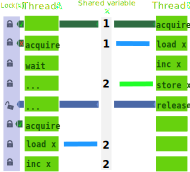
\includegraphics[width=0.7\textwidth]{Illustrations/Lock}
		\label{fig:lock}
	\end{figure}
\end{frame}

\section[Thread Scheduling]{Thread Scheduling on Linux}
\subsection[CFS]{Completely Fair Scheduler}
\begin{frame}
\frametitle{Completely Fair Scheduler (CFS)}

\begin{itemize}
\item Default Linux thread scheduler (there are others)
\item Handles which threads are executed at what times on this core
\item Spend a \emph{fair} amount of runtime on all threads
\end{itemize}

\end{frame}


\begin{frame}
\frametitle{Completely Fair Scheduler (CFS)}

\begin{itemize}
\item Like any program, runs on one core
\item Makes sure all threads run \emph{at least once} within an arbitrary interval of CPU~cycles
\item Distribute \emph{timeslices} (max CPU cycles) among threads
\item Threads with higher priority (weights) get larger timeslices
\item Monitors the number of cycles that the running thread receives and switches it out when it exceeds its timeslice
\end{itemize}

\begin{figure}
		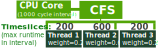
\includegraphics[width=0.8\textwidth]{Illustrations/CFS}
		\label{fig:cfs}
\end{figure}

\linespace

\end{frame}

\begin{frame}
\frametitle{Runqueues}

\begin{itemize}
	\item The data structure within the CFS that contains threads is called a runqueue
	\item A \emph{runqueue} is a priority queue that sorts for threads that have received the least cycles in the current interval
	\item When a thread reaches its maximum time, the first thread in the runqueue is chosen to replace
\end{itemize}

\end{frame}




\begin{frame}
\frametitle{Runqueues on Multiple Cores}
If each core needs work to do, how are threads distributed?

\linespace

Before we can answer this question, we need to know some about switching threads, cache and processor state

\end{frame}



\subsection[Cache]{Thread State and Cache}

\begin{frame}
\frametitle{Context Switching}
\begin{itemize}
\item The scheduler \emph{switches} active threads on cores by saving and restoring thread and processor state information.
\item These switches are called \emph{context switches}
\item Scheduler performance 
\end{itemize}
\end{frame}

\begin{frame}
\frametitle{Process and Thread State}

Process State

\begin{itemize}
	\item[] Consists of resources that each of its threads should have access to including compiled code, and data.
\end{itemize}

Thread State

\begin{itemize}
	\item[] Scheduler uses this information to pause and resume a thread's execution
\end{itemize}

\end{frame}


\begin{frame}
\frametitle{Cache}

\begin{columns}
\begin{column}{0.5\textwidth}
\begin{itemize}
	\item Memory and cache exists in a hierarchy %POINT ON SLIDE L1, L2, Last-level cache
	\item How cache is arranged depends on the machine:
	\begin{itemize}
		\item A cache can exist \emph{on}, \emph{built-in} to, or \emph{outside} a processor
		\item Cache can be one per \emph{n} processors or one per \emph{n} cores
	\end{itemize}
\end{itemize}

\end{column}
\begin{column}{0.5\textwidth}
		\begin{figure}
		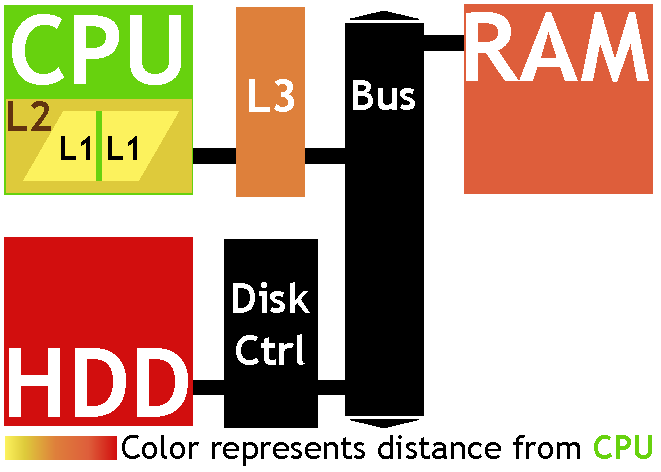
\includegraphics[width=0.95\textwidth]{Illustrations/CacheAbstract}
		\label{fig:domains}
		\caption{Distance of various forms of memory from CPU}
		\end{figure}
	\end{column}
\end{columns}
\end{frame}

\begin{frame}
\frametitle{Cache}

\begin{columns}
\begin{column}{0.5\textwidth}
\begin{itemize}
	\item \emph{Locality}: Speed of memory read and writes decrease as distance from CPU increases
	\item Cache is the fastest form of memory
	
	\linespace
	
	\item \emph{Cache coherence:} Any changes to memory shared by two caches must propogate to the other to maintain correctness
\end{itemize}

\end{column}
\begin{column}{0.5\textwidth}
		\begin{figure}
		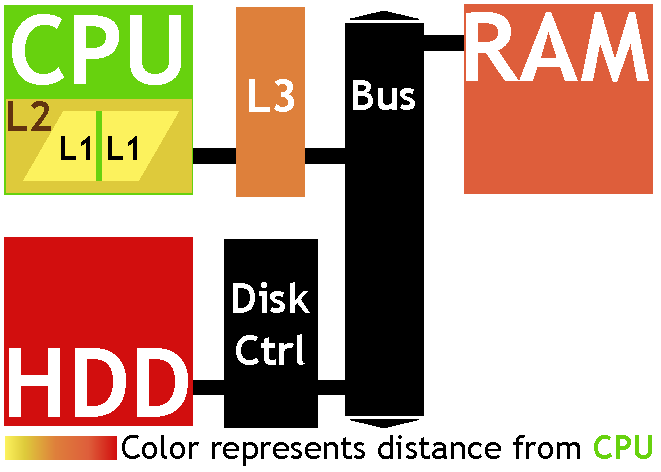
\includegraphics[width=0.95\textwidth]{Illustrations/CacheAbstract}
		\label{fig:domains}
		\caption{Distance of various forms of memory from CPU}
		\end{figure}
	\end{column}
\end{columns}
\end{frame}


\begin{frame}
\frametitle{Runqueues on Multiple Cores (Revisited)}

Since process states are heaver than thread states, context switches between threads of different processes are more expensive

\linespace

\begin{itemize}
	\item If all cores shared one runqueue, access and changes to it would need to be synchronous and cache-coherent
	\item This would slow the system to a crawl
	\item So each core has its own runqueue and threads
\end{itemize}

\linespace

\begin{itemize}
\item In order to best take advantage of available cores, the load on each of the core's runqueues must stay balanced.
\item Most schedulers, including the CFS periodically run a load-balancing algorithm
\end{itemize}
\end{frame}

\section[New Schedulers]{Two new schedulers}


\begin{frame}

\frametitle{Shuffler and FLSCHED}

\linespace

Both schedulers aim to solve the same problem, but for different processor types.

\linespace

\begin{table}

\begin{tabular}{l c l}
Shuffler & $\rightarrow$ & multiprocessor multicore \\
FLSCHED & $\rightarrow$ & single-chip manycore processor\\
\end{tabular}

\end{table}

\linespace
\textbf{Problem:} As you add more threads to parallel computing problems, they start to operate slower rather than faster!

\linespace

The term for what these systems face is called \emph{lock contention} and it is to blame for the high acquisition times.

\end{frame}

\subsection{Shuffler}
\begin{frame}
\frametitle{Shuffler}

By researchers Kumar et al.

\linespace


\end{frame}
\begin{frame}

(in short, unfinished)

Shuffler
\begin{itemize}

\item Monitors the lock acquisition times of various executing threads
\item Isolates groups of threads that have similar lock acquisition times, and migrate those threads to the same processor, assuming that those groups of threads may be contending with eachother for the same lock and would both have faster acquisition times if they were colocated.
\end{itemize}

\end{frame}

\subsection{FLSCHED}
\begin{frame}
\frametitle{FLSCHED}

(in short, unfinished)

Designed by Jo et al. with manycore processors (specifically the Xeon Phi) in mind.

\linespace

The Xeon and Xeon Phi manycore processors come with varying degrees of cores, from 24 to 76 cores. With such potential for parallelism and as the number of cores rise, any small hitch in a critical system component can lead to significant performance degradation. 

The hithces that they isolated were due to locks emplaced by features and requirements of the CFS scheduler.

\end{frame}

\begin{frame}
\frametitle{One requirement to rule them all: EFFICIENCY!!!}

FLSCHED Aims to improve the efficiency by removing all locks from the scheduler component. In order to do this, they gutted the requirements and features of the CFS scheduler and simplified.

\linespace

The requirements that they removed are:

\begin{itemize}
\item Fairness,
\item Responsiveness,
\end{itemize}

The features that they removed were:

\begin{itemize}
\item Group scheduling
\end{itemize}

\end{frame}

\begin{frame}
FLSCHED is a scheduler implementation without any locks\footnote{In Jo et al. they clarify it is still built on top of the \emph{scheduler core} which still locks in it.}.

\linespace
Lock contention may exist in FLSCHED, but it isn't a problem in the same way as in Shuffler because none of the cores exist on other processors, there is only one processor, so that latency is not a concern.

\end{frame}

\section[Conclusions]{Conclusions}

\begin{frame}
\frametitle{Conclusions}

todo

\end{frame}

\begin{frame}
\frametitle{Thanks!}

Thank you for your time and attention!

\begin{center}
{\huge Questions?}
\end{center}
\end{frame}

\section*{References}

\begin{frame} 
\frametitle{References} 

\begin{thebibliography}{lskdjf}

\bibitem{Jo:2017}
H.~Jo, W.~Kang, C.~Min, and T.~Kim.

\newblock FLsched: A lockless and lightweight approach to OS scheduler for Xeon Phi.

\newblock In G\"unther Raidl, \emph{et al}, editors, {\em GECCO '09}, pages 1019--1026, Montr\'eal, Qu\'ebec, Canada, 2009.

\bibitem{Lozi:2016}
R.~Poli and N.~McPhee.
\newblock A linear estimation-of-distribution {GP} system.
\newblock In M.~O'Neill, \emph{et al}, editors, {\em EuroGP 2008}, volume
  4971 of {\em LNCS}, pages 206--217, Naples,
  26-28 Mar. 2008. Springer.
  
\end{thebibliography}

\linespace
\begin{center}
	See the GECCO '09 paper for additional references.
	\end{center}
\end{frame} 

\end{document}


